\chapter{刚体运动的动能}

\section{刚体的独立坐标}

刚体系统具有$N$个粒子,这些粒子间的相对位置是确定的,也就是说对于任意两个粒子$i$和$j$,其
相对距离满足
\begin{equation}
	r_{ij} = c_{ij}	\label{eq:rigid-constraint}
\end{equation} 
其中$c_{ij}$是一个常数。这是$N$粒子刚体系统满足的约束方程。确定这样一个系统的空间状态,我
们需要确定$N$个粒子的自由度,整个系统总共就有$3N$个自由度,这是非常复杂的,而上式所确定的
约束方程总共有$\dfrac{N(N-1)}{2}$个,对于很大的$N$来说,这远远大于了系统的所有粒子的自由度
数目,因此上述的约束方程并不是完全独立的。

在确定整个刚体系统的空间位置前,我们先考虑如何确定一个点在空间中的位置。对于空间中一个点$4$
的位置,我们可以先确定空间中不同直线上的三个点$1$、$2$、$3$的位置,并且确切地知道点$4$相对
于这三个点的距离时,我们就可以唯一确定点$4$的位置。现在考虑多粒子系统的刚体系统,我们可以
知道任意一点$i$相对于$1$、$2$、$3$的距离$c_{i1}$、$c_{i2}$、$c_{i3}$,这样,我们基于这三个
点就可以确定刚体内其余所有点的位置,也就确定了这个刚体的空间位置。

现在,我们已经把整个刚体的空间位置由$N$个点的自由度约化成了确定$3$个点的自由度问题,下面来
定出这$3$个点所需要的自由度个数。首先,我们知道了刚体内所有点的约束条件为式\eqref{eq:rigid-constraint},
从而知道这三个点具有确定的相对距离为
\begin{equation*}
	r_{12} = c_{12}, \quad r_{13} = c_{13}, \quad r_{23} = c_{23}
\end{equation*} 
我们确定点$1$需要三个自由度;点$2$在以点$1$为球心,$r_{12}$为半径的球面上,因此我们只需要
知道点$2$的两个自由度便可以确定其位置;在确定前两个点的位置后,点$3$位于点$1$和点$2$为球心,
$r_{13}$和$r_{23}$为半径的球面相交所构成的圆上,因此,我们只需要确定其中一个自由度就可以知
道点$3$的确定位置。综上,我们总共需要确定$3+2+1=6$个自由度便可以最终定下三个点的具体空间位
置,再根据刚体内点的约束关系,就可以确定好整个系统的空间位置。

\paragraph*{相对坐标系统}
\begin{figure}[htbp]
	\centering
	\begin{tikzpicture}
    \draw[-Stealth, line width=1pt]             (0, 0) -- (4, 0);
    \draw[-Stealth, line width=1pt, rotate=90]  (0, 0) -- (4, 0);
    \draw[-Stealth, line width=1pt, rotate=225]  (0, 0) -- (3, 0);

    \node at (4, 0)  [below] {$y$};
    \node at (0, 4)  [left] {$z$};
    \node at (-2, -2) [left] {$x$};
\end{tikzpicture}

	\label{fig:relative-coord}
\end{figure}
空间中有一套Cartesian坐标系统,刚体处于这个坐标系统中,称为unprimed坐标系统,单位矢量为
$\vbe_{i}$、$\vbe_{j}$和$\vbe_{k}$;在刚体内部建立另一套Cartesian坐标系统,刚体内部的粒子用此坐标系统来标记,称为primed坐标系统,其单位矢量为$\vbe_{i}^{\,\prime}$、$\vbe_{j}^{\,\prime}$和$\vbe_{k}^{\,\prime}$。那么,unprimed和primed就是两套相对的坐标系统,若我们需要知道刚体中某个粒子的状态,我们只需要知道这个粒子在primed坐标系中的状态,再知道primed相对于unprimed坐标系中的状态,就可以确定刚体中的粒子运动。

矢量不会因为我们改变坐标系统而改变其空间分布,因此两个坐标系统中观察到的是同一个矢量,故
\begin{equation}
	\vbr = x \vbe_{i} + y \vbe_{j} + z \vbe_{k}
	     = x^{\prime} \vbe_{i}^{\,\prime} + y^{\prime} \vbe_{j}^{\,\prime} + z^{\prime} \vbe_{k}^{\,\prime}
\end{equation}
利用上式,对矢量的描述中,从unprimed坐标变换到primed坐标的矢量分量变换为:
\begin{equation}
	\begin{aligned}
		x^{\,\prime} =& \cos{\theta_{11}} x + \cos{\theta_{12}} y + \cos{\theta_{13}} z \\
		y^{\,\prime} =& \cos{\theta_{21}} x + \cos{\theta_{22}} y + \cos{\theta_{23}} z \\
		z^{\,\prime} =& \cos{\theta_{31}} x + \cos{\theta_{32}} y + \cos{\theta_{33}} z
	\end{aligned}
\end{equation}
由正交关系($\alpha$、$\beta$遍历$i$、$j$、$k$)
\begin{equation}
	\vbe_{\alpha} \cdot \vbe_{\beta} = \delta_{\alpha\beta}
	\quad
	\vbe_{\alpha}^{\,\prime} \cdot \vbe_{\beta}^{\,\prime} = \delta_{\alpha\beta}^{\,\prime}
\end{equation}
并结合以上两式,我们可以得到两坐标系统单位矢量间的变换关系:
\begin{enumerate}
	\item 从primed坐标变换到unpried坐标,满足
		\begin{equation}
			\begin{aligned}
				\vbe_{i}^{\,\prime} =& \cos{\theta_{11}} \vbe_{i} + \cos{\theta_{12}} \vbe_{j} + \cos{\theta_{13}} \vbe_{k} \\
				\vbe_{j}^{\,\prime} =& \cos{\theta_{21}} \vbe_{i} + \cos{\theta_{22}} \vbe_{j} + \cos{\theta_{23}} \vbe_{k} \\
				\vbe_{k}^{\,\prime} =& \cos{\theta_{31}} \vbe_{i} + \cos{\theta_{32}} \vbe_{j} + \cos{\theta_{33}} \vbe_{k}
			\end{aligned}
		\end{equation}
	\item 从umprimed坐标变换到primed坐标,满足
	\begin{equation}
		\begin{aligned}
			\vbe_{i} =& \cos{\theta_{11}} \vbe_{i}^{\,\prime} + \cos{\theta_{21}} \vbe_{j}^{\,\prime} + \cos{\theta_{31}} \vbe_{k}^{\,\prime} \\
			\vbe_{j} =& \cos{\theta_{12}} \vbe_{i}^{\,\prime} + \cos{\theta_{22}} \vbe_{j}^{\,\prime} + \cos{\theta_{32}} \vbe_{k}^{\,\prime} \\
			\vbe_{k} =& \cos{\theta_{13}} \vbe_{i}^{\,\prime} + \cos{\theta_{23}} \vbe_{j}^{\,\prime} + \cos{\theta_{33}} \vbe_{k}^{\,\prime}
		\end{aligned}
	\end{equation}
	\item 方向角的正交关系为
		\begin{equation}
			\sum_{l = 1}^{3} \cos{\theta}_{lm^{\prime}} \cos{\theta}_{lm} = \delta_{mm^{\prime}}
		\end{equation}
\end{enumerate}

\paragraph*{正交变换}
现在,用$x_1$、$x_2$、$x_3$分别表示$x$、$y$和$z$,方向余弦重新表述如下
\begin{equation}
	a_{ij} = \cos{\theta_{ij}}
\end{equation}
有如下关系成立
\begin{equation}
	\left\{\begin{aligned}
	x_1^{\prime} =& a_{11}x_1 + a_{12}x_2 + a_{13}x_3 \\
	x_2^{\prime} =& a_{21}x_1 + a_{22}x_2 + a_{23}x_3 \\
	x_3^{\prime} =& a_{31}x_1 + a_{32}x_2 + a_{33}x_3
	\end{aligned}\right. \qquad
	\left\{\begin{aligned}
		x_1 =& a_{11}x_1^{\prime} + a_{12}x_2^{\prime} + a_{13}x_3^{\prime} \\
		x_2 =& a_{21}x_1^{\prime} + a_{22}x_2^{\prime} + a_{23}x_3^{\prime} \\
		x_3 =& a_{31}x_1^{\prime} + a_{32}x_2^{\prime} + a_{33}x_3^{\prime}
	\end{aligned}\right.
\end{equation}
根据爱因斯坦求和规则$\sum_{i}x_i^2 \rightarrow x_i x_i$,将前面的方向角正交关系重新表述如下:
\begin{equation}
	a_{ij} a_{ik} = \delta_{jk}
\end{equation}
\begin{note}
	满足上述关系的变换矩阵成为正交变换,此为判定矩阵是否为正交矩阵的充要条件。
\end{note}

若primed和unprimed坐标系间可通过正交变换实现转换,相应的的变换矩阵为
\begin{equation}
	\underbrace{
	\begin{bmatrix}
		a_{11}	&	a_{12}	&	a_{13} \\
		a_{21}	&	a_{22}	&	a_{23} \\
		a_{31}	&	a_{32}	&	a_{33}
	\end{bmatrix}
	}_{\text{unprimed to primed}}
	\qquad
	\underbrace{
	\begin{bmatrix}
		a_{11}	&	a_{21}	&	a_{31} \\
		a_{12}	&	a_{22}	&	a_{32} \\
		a_{13}	&	a_{23}	&	a_{33}
	\end{bmatrix}
	}_{\text{primed to unprimed}}
\end{equation}

%%%%%%%%%%%
\paragraph*{矢量在不同坐标系下的变换}
现有两套坐标系,分别为primed和unprimed,它们对对空间中的同一个矢量的表示应该是等价的,即
\begin{equation}
	(\vec{r})^{\prime} = A \vec{r}
\end{equation}
上式等号坐标,对矢量加上括号表示这个矢量在primed坐标系下表示;等号右边的$A$表示不同坐标系间的变换矩阵,未加括号的$\vec{r}$实在unprimed坐标系下的表示。上面的式子的物理含义为:$\vec{r}$是矢量在unprimed坐标系下的表达,现在我们想要在primed坐标系下对这个矢量进行重新表述,我们就需要将坐标系进行变换,而$A$的作用就是将primed坐标系转到unprimed坐标系,此时,这个矢量在新的坐标系下的表示就是$(\vec{r})^{\prime}$。

此外,相对的,坐标系间的变换也可以理解成在同一坐标系下对某一个矢量进行变换,即
\begin{equation}
	\vec{r}^{\prime} = A \vec{r}
\end{equation}

%%%%%%%%%%%%%%%%%%%%%%%%
\section{变换矩阵的形式特性}
\paragraph*{变换矩阵的一般性质}
矩阵变换具有先后顺序性,对矢量$\vec{r}$先进行变换$B$得到$\vec{r}^{\prime}$,再对$\vec{r}^{\prime}$进行变换$A$得到矢量$\vec{r}^{\prime\prime}$,则对应的变换为
\begin{equation}
	\vec{r}^{\prime\prime} = C\vec{r} = A\vec{r}^{\prime} = A(B\vec{r}) = AB\vec{r}
\end{equation}
这里定义
\begin{equation}
	C = AB \quad (\text{一般的,}AB\neq BA)
\end{equation}
$AB$和$BA$表示不同的操作,一般不相等,除非其中一个为单位矩阵(意味着这个变换对矢量不做任何变换)。$C$的矩阵元为
\begin{equation}
	C_{ij} = a_{ik}b_{kj} \quad (\text{爱因斯坦求和规则})
\end{equation}

若有多个矩阵变换操作,则表示为对应的矩阵乘法,且有
\begin{equation}
	(AB)C = A(BC)
\end{equation}

现在unprimed坐标系下有一矢量$\vec{f}$,经变换矩阵$A$作用后变为矢量$\vec{g}$,即
\begin{equation}
	\vec{g} = A \vec{f}
\end{equation}
变换矩阵$B$的作用是将unprimed坐标系变为primed坐标系,此时primed坐标系下的矢量$\vec{g}$表示为
\begin{equation}
	B\vec{g} = B(A\vec{f}) = (BAB^{-1})(B\vec{f})
\end{equation}
其中,$B\vec{f}$是矢量$\vec{f}$在primed坐标系下的表示;$BAB^{-1}$为primed坐标系下的变换矩阵$A$(在unprimed坐标系下作用到矢量上)的表示,换句话就是说$BAB^{-1}$和$A$对矢量的操作是一样的,只不过它们在不同的坐标系下进行操作,$BAB^{-1}$是在primed坐标系下对矢量的操作,而$A$实在primed坐标系下对矢量的操作。以上两式结合来看,表示了矢量变换在不同坐标系统下的变换操作。


\paragraph*{变换为正交矩阵的情况}
若矩阵$A$为正交矩阵,则$A$的逆$A^{-1}$与其转置$\tilde{A}$等价,满足以下等式
\begin{equation}
	\begin{aligned}
		A^{-1} &= \tilde{A} \\
		\tilde{A}A = A^{-1}&A = AA^{-1} = \bm{1}
        \label{eq:orth-mat-qualification}
	\end{aligned}
\end{equation}
以上推得正交矩阵行列式的规则
\begin{equation}
	|A|^2 = |\tilde{A}A| = |\tilde{A}|\cdot|A| = 1
\end{equation}

%%%%%%%%%%%%%%%%%%%%%%%%
\section{Euler角}
\CJKunderline{欧拉角可以描述一个物体定点转动,也可以描述两个坐标系之间的转动变换,其转动矩阵的行列式的值为$+1$。}欧拉角有$x$-convention和$y$-convention两种,其常用领域有所不同。

\subsection{\texorpdfstring{$x-$}convention下的Euler角}
$x$-convetion的欧拉角操作如\cref{fig:x-euler-ang}所示。欧拉角变换可分3步进行操作:
\begin{enumerate}
    \item 从初始的笛卡尔坐标$xyz$开始,先绕$z$轴转动角度$\phi$(转动后的主轴重新标定为$x\rightarrow\xi$、$x\rightarrow\eta$和$z\rightarrow\zeta$),对应的变换矩阵为$\bm{A}$;
    \item 绕主轴$\xi$转动角度$\theta$,转动后的主轴重新进行标定($\xi\rightarrow\xi^{\prime}$、$\eta\rightarrow\eta^{\prime}$和$\zeta\rightarrow\zeta^{\prime}$),对应的变换矩阵为$\bm{B}$;
    \item 最后一次是绕$\zeta^{\prime}$转动角度$\psi$,此时主轴变为$x^{\prime}\rightarrow z^{\prime}$、$\eta^{\prime}\rightarrow y^{\prime}$和$\zeta^{\prime}\rightarrow z^{\prime}$,对应的变换矩阵为$\bm{C}$。
\end{enumerate}
\begin{figure}[htb]
    \centering
    \setlength{\abovecaptionskip}{0.2cm}
    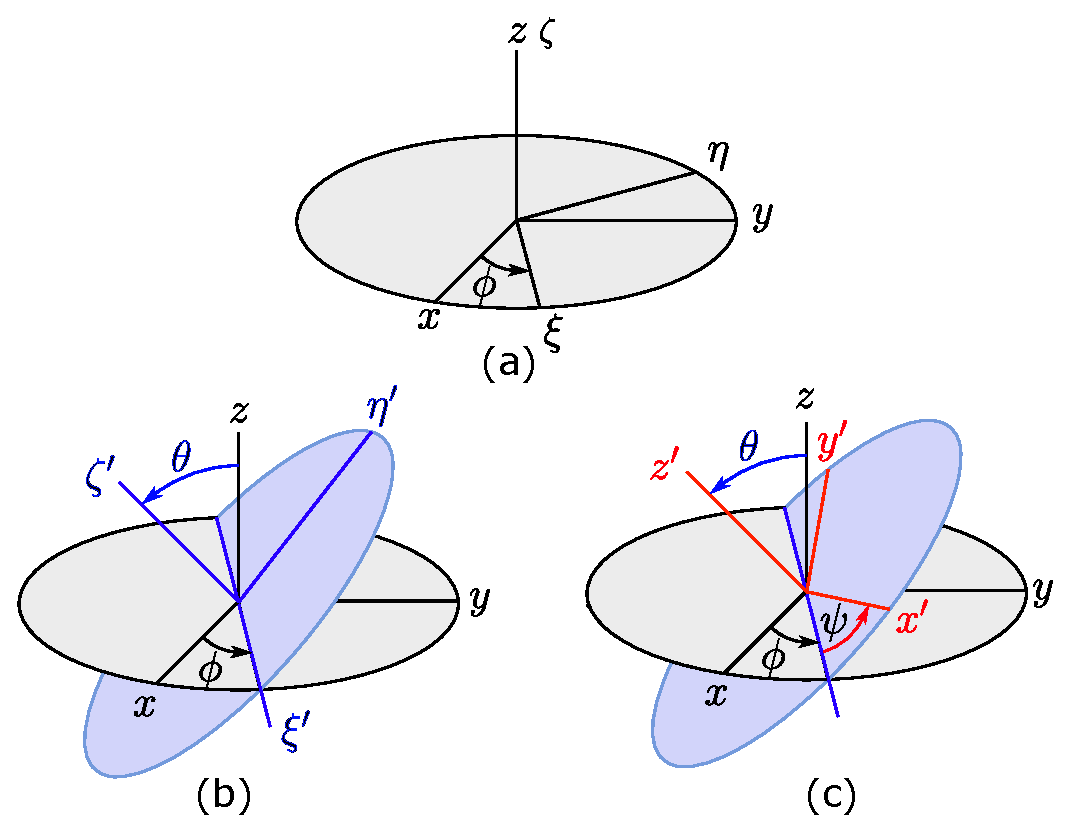
\includegraphics[scale=0.6]{./figure/classical-mechanics/Eular-angle.eps}
    \caption{$x$-convention的欧拉角。}
    \label{fig:x-euler-ang}
\end{figure}

通过完成上述操作,我们最终实现从$xyz\rightarrow x^{\prime}y^{\prime}z^{\prime}$的空间转换。以上操作也可以通过某一个转动变化直接实现,其对应的变换矩阵为$\bm{R}$,则应有如下关系成立:
\begin{equation}
    \bm{R} = \bm{CBA}
\end{equation}
\begin{note}
    这里的物理意义很明显,这些矩阵均表示一个转动操作,我们直接将其作用的$xyz$坐标系的基矢上,会发现$\bm{Ax}$作用后得到$\xi\eta\zeta$坐标系下的基矢,即
    \begin{equation*}
        \begin{pmatrix}
            \vec{\bm{e}}_{\xi} \\
            \vec{\bm{e}}_{\eta} \\
            \vec{\bm{e}}_{\zeta} \\
        \end{pmatrix}
        =  \bm{A}
        \begin{pmatrix}
            \vec{\bm{e}}_{x} \\
            \vec{\bm{e}}_{y} \\
            \vec{\bm{e}}_{z} \\
        \end{pmatrix}
    \end{equation*}
\end{note}

$\bm{A}$矩阵对应为绕$z$轴的旋转,$\bm{B}$为绕$\xi$轴的转动,$\bm{C}$为绕$\zeta^{\prime}$轴的转动,其对应的变换为
\begin{equation}
    \bm{A} = \begin{pmatrix}
        \cos{\phi} & \sin{\phi} & 0 \\
        -\sin{\phi} & \cos{\phi} & 0 \\
        0          & 0          & 0
    \end{pmatrix}
    \quad
    \bm{B} = \begin{pmatrix}
        1           & 0             & 0 \\
        0           & \cos{\theta}  & \sin{\theta} \\
        0           & -\sin{\theta} & \cos{\theta}
    \end{pmatrix}
    \quad
    \bm{C} = \begin{pmatrix}
        \cos{\psi} & \sin{\psi} & 0 \\
        -\sin{\psi} & \cos{\psi} & 0 \\
        0          & 0          & 0
    \end{pmatrix}
\end{equation}
因此,矩阵$R$为
\begin{equation}
    \bm{R} = \bm{CBA}
           = \begin{pmatrix}
            \cos{\psi}\cos{\phi} - \cos{\theta}\sin{\phi}\sin{\psi} & \cos{\psi}\sin{\phi} + \cos{\theta}\cos{\phi}\sin{\psi} & \sin{\psi}\sin{\theta} \\
            -\sin{\psi}\cos{\phi} - \cos{\theta}\sin{\phi}\cos{\psi} & -\sin{\psi}\sin{\phi} + \cos{\theta}\cos{\phi}\cos{\psi} & \cos{\psi}\sin{\theta} \\
            \sin{\theta}\sin{\phi} & -\sin{\theta}\cos{\phi} & \cos{\theta}
           \end{pmatrix}
		   \label{eq:Euler-rot-mat}
\end{equation}

这里,$\bm{R}$为正交矩阵,其逆矩阵表示从$x^{\prime}y^{\prime}z^{\prime}$变换回$xyz$坐标系,根据\cref{eq:orth-mat-qualification},有
\begin{equation}
    \bm{R}^{-1} = \tilde{\bm{R}}
\end{equation}

%%%%%%%%%%%%%%%%%%%%%%%%
\subsection{刚体运动中的Euler角}
当刚体随时间发生,其变换矩阵$\bm{R}$也是关于时间的连续函数$\bm{R}(t)$。以下讨论基于$x$-convention下的欧拉角。
\begin{theorem}[Euler定理]
    固定一点的刚体的广义位移相当于刚体绕某一根轴的转动。
\end{theorem}

首先计算矩阵$\bm{R}$的本征值,将其作用到$xyz$的某一矢量上,对应的久期方程(或本征方程)为
\begin{equation}
    \vec{\bm{r}}^{\,\prime} = \bm{R}\vec{\bm{r}} = \lambda\vec{\bm{r}}
\end{equation}
\begin{note}
    这个方程作用在$xyz$坐标系下表示的矢量$\vec{\bm{r}}$上,最后得到的矢量$\lambda\vec{\bm{r}}$依旧是用$xyz$坐标表示的,这表明本征方程中的矩阵$\bm{R}$的作用效果是坐标系自己和自己之间的变换,或者是对矢量$\vec{\bm{r}}^{\,\prime}$自己的操作。
\end{note}

上面的久期方程有非平庸解的条件是其行列式为0
\begin{equation}
    \begin{vmatrix}
        r_{11} - \lambda & r_{12}           & r_{13} \\
        r_{21}           & r_{22} - \lambda & r_{23} \\
        r_{31}           & r_{32}           & r_{33} - \lambda \\
    \end{vmatrix}
    = 0
    \label{eq:vec-tran-mat}
\end{equation}
\begin{note}
    由于$\bm{R}$是正交矩阵,描述的是一种转动,欧拉定理指出其必定有本征值$\lambda = +1$,表示其经过转动不变。
\end{note}
下面对式\cref{eq:vec-tran-mat}进行求解。首先做一些定义:


%%%%%%%%%%%%%%%%%%%%%%%%
\section{无穷小转动}
刚体无穷小转动时,其Euler角变化趋于0,即
\begin{equation*}
	\theta\rightarrow 0, \quad \phi\rightarrow 0, \quad \psi\rightarrow 0
\end{equation*}
取极限有
\begin{equation*}
	d\theta \equiv \lim_{\theta\rightarrow 0} \theta = \lim_{\theta\rightarrow 0} \sin{\theta}, \quad \lim_{\theta\rightarrow 0} \cos{\theta} = 1
\end{equation*}
上述关系对$\phi$和$\psi$同时成立,根据\cref{eq:Euler-rot-mat},忽略高阶无穷小,这样,无穷小Euler转动角对应的变换矩阵$\bm{R}$可写为
\begin{equation}
	\bm{R} = \begin{pmatrix}
		1                 &  (d\phi + d\psi)  &    0 \\
		-(d\phi + d\psi)  &  1                & d\theta \\
		0                 &  - d\theta        & 1
	\end{pmatrix}
\end{equation}
